\section{Introduction}

\subsection{Problem}
\begin{frame}{Problem}{Lack of mature frameworks/DSLs for system testing}
  \begin{itemize}
  \item \textbf{Dearth} of mature frameworks and tools available for system testing
  \item Existing Frameworks: \textbf{Not suitable} for system testing
  \item \textbf{Pressing} need for system level testing
  \end{itemize}
\end{frame}

\begin{frame}{Existing Testing Frameworks}
\begin{figure}[h!]
  \centering
    
\includegraphics[height=50px]{figures/selenium.jpg}
    
\includegraphics[height=50px]{figures/junit-logo.png}
\end{figure}
\begin{figure}[h!]
  \centering
    
\includegraphics[height=100px]{figures/scalaTest.jpg}
\end{figure}
\end{frame}

\begin{frame}{Types of System Testing}
\begin{figure}[h!]
  \centering
    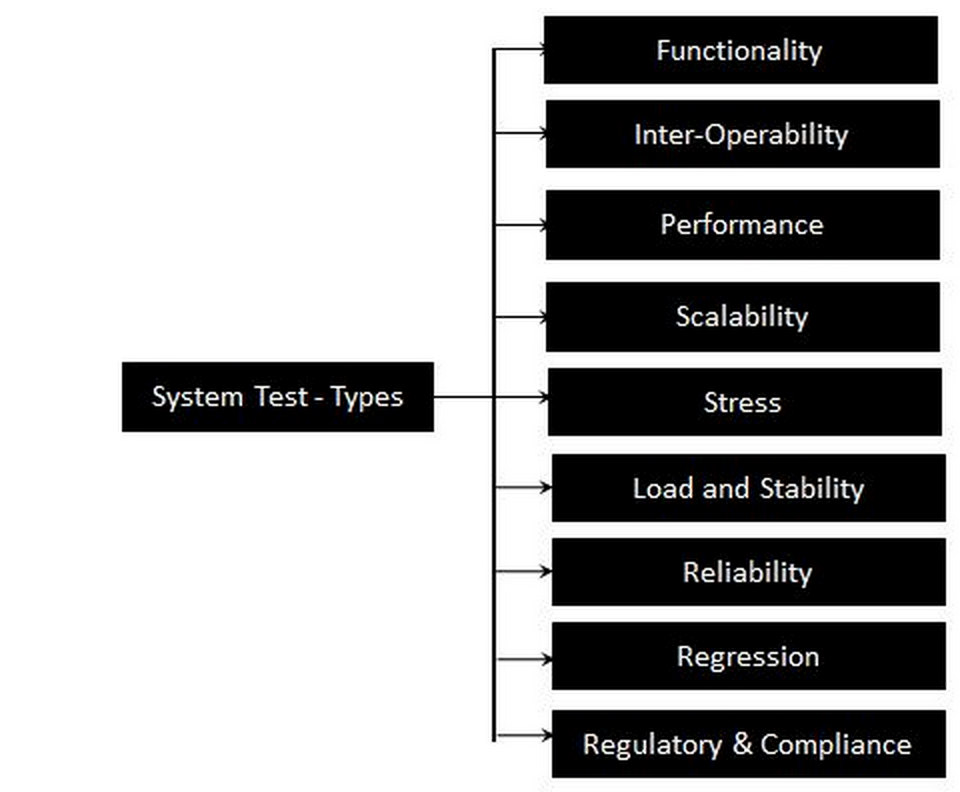
\includegraphics[height=180px]{figures/system_testing_types.png}
  \caption{Different types of system testing}
\end{figure}
\end{frame}

\begin{frame}{Case Study for System Testing: Language Verification}
Requirements:
\begin{itemize}
  \item {HIP Verification}
  \item {SLEEK Verification}
  \item {HIP/SLEEK Regression Testing}
  \item {HIP/SLEEK Verifier Performance Testing}
  \item {HIP/SLEEK Code Base Repository Testing}
  \item {Programming Language Prover Testing}
  \end{itemize}
\end{frame}

\begin{frame}{Existing System for HIP/SLEEK verification - Perl Script}
    \begin{figure}[H]
  \centering
    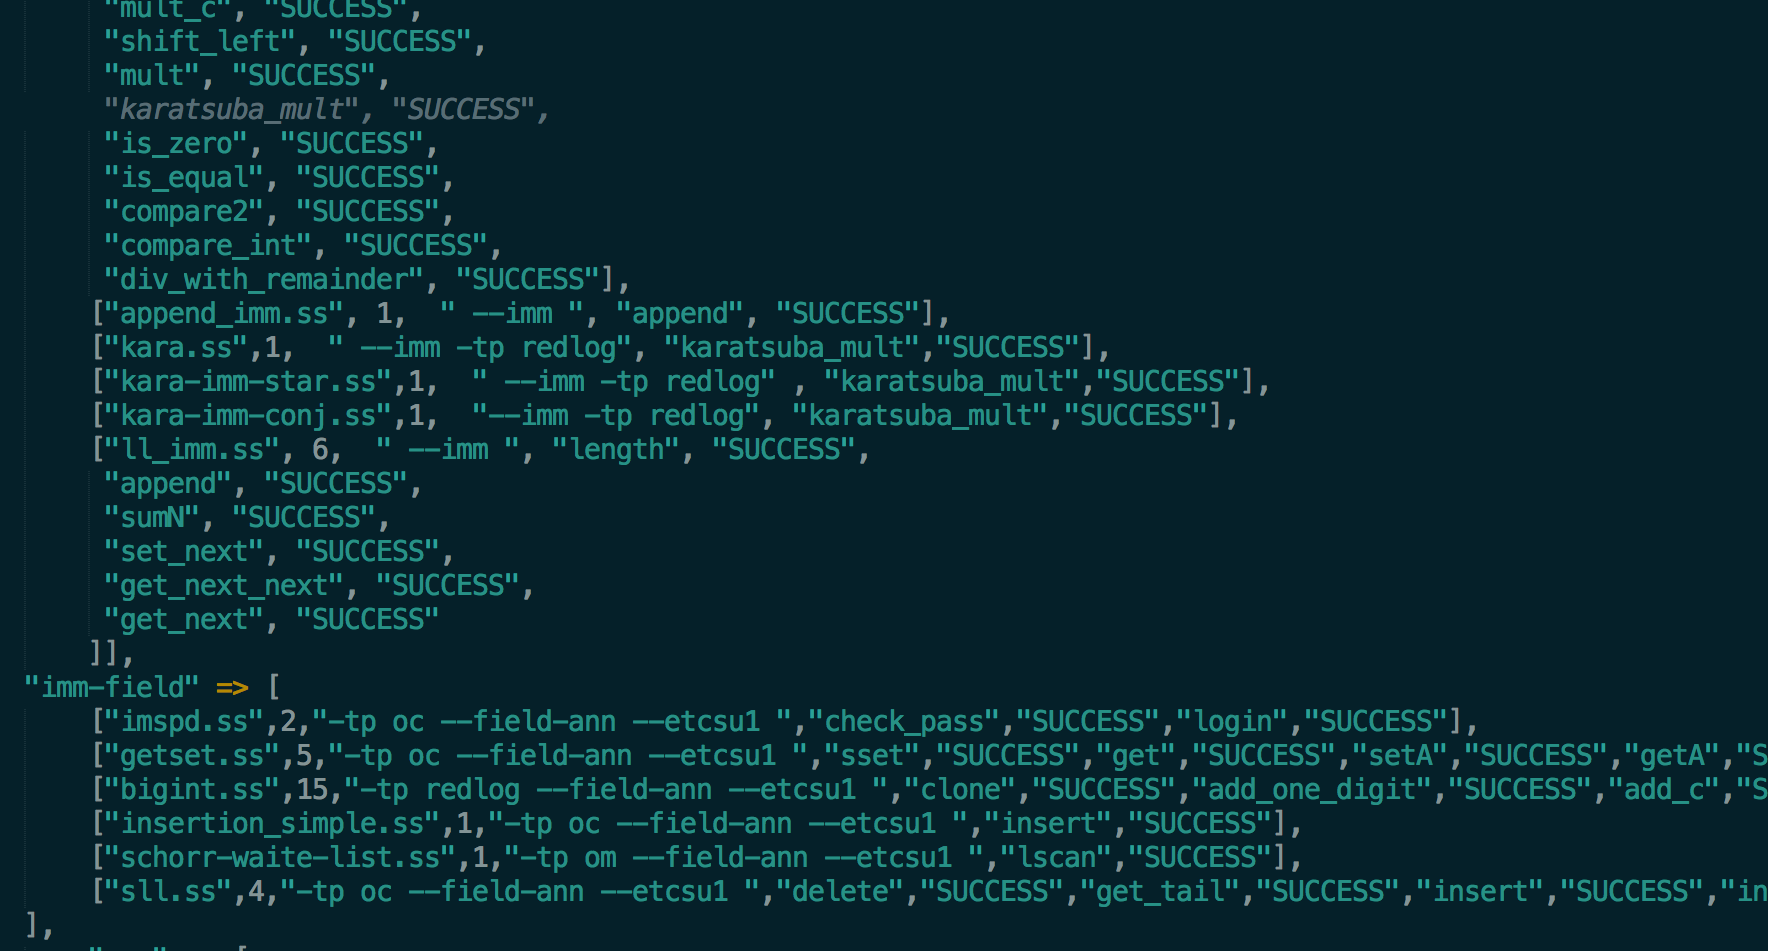
\includegraphics[width=320px]{figures/legacy1.png}
  \caption{Legacy Perl Script}
\end{figure}
\end{frame}

\begin{frame}{Existing System for HIP/SLEEK verification - Perl Script}
    \begin{figure}[H]
    \centering
    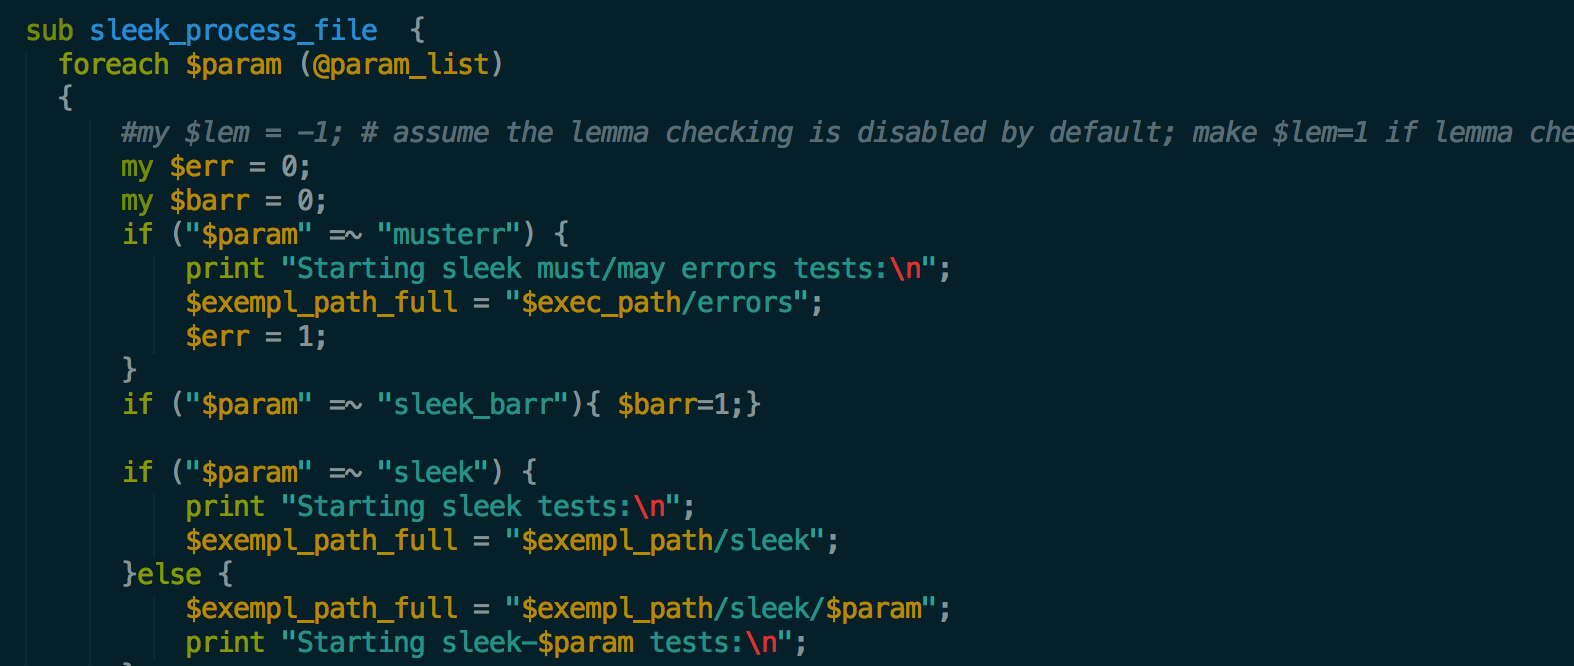
\includegraphics[width=320px]{figures/legacy2.png}
  \caption{Legacy Perl Script}
\end{figure}
\end{frame}

\subsection{Solution}
\begin{frame}{Overview of Solution}
The DSL written covers \textbf{Performance Testing, Regression Testing, Functional Testing and Repository Testing}.
\begin{figure}[h!]
  \centering
    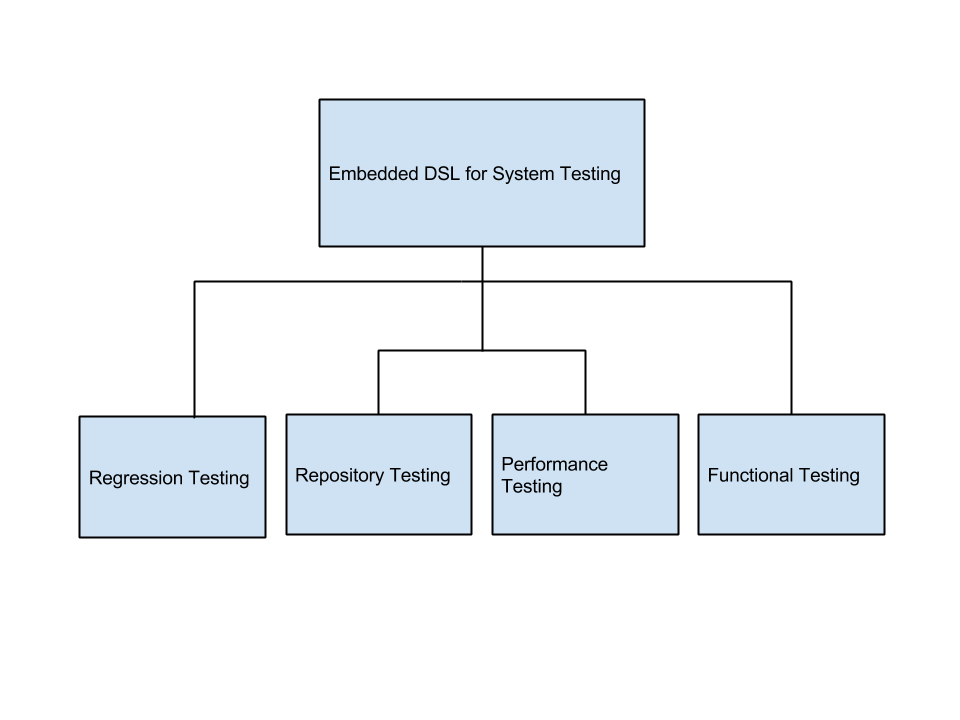
\includegraphics[height=160px]{figures/overview_of_solution.png}
\end{figure}
\end{frame}

\begin{frame}{New System - DSL developed}
\begin{figure}[H]
  \centering
    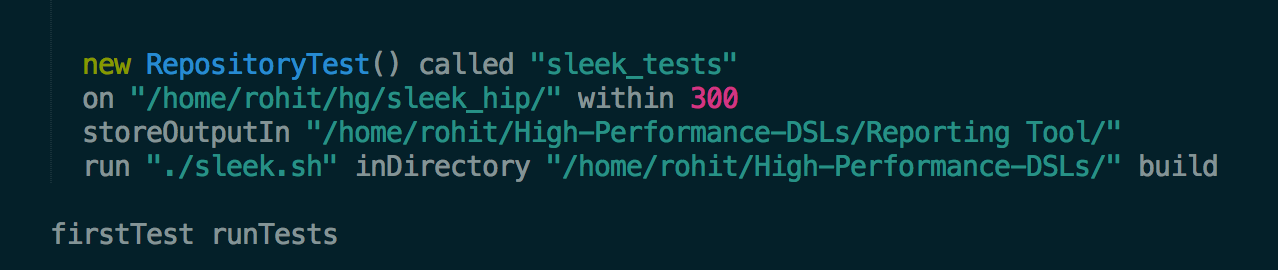
\includegraphics[width=320px]{figures/reportingDSL.png}
  \caption{Individual Test Case Creation}
\end{figure}
\end{frame}

\begin{frame}{New System - DSL developed}
\begin{figure}[H]
  \centering
    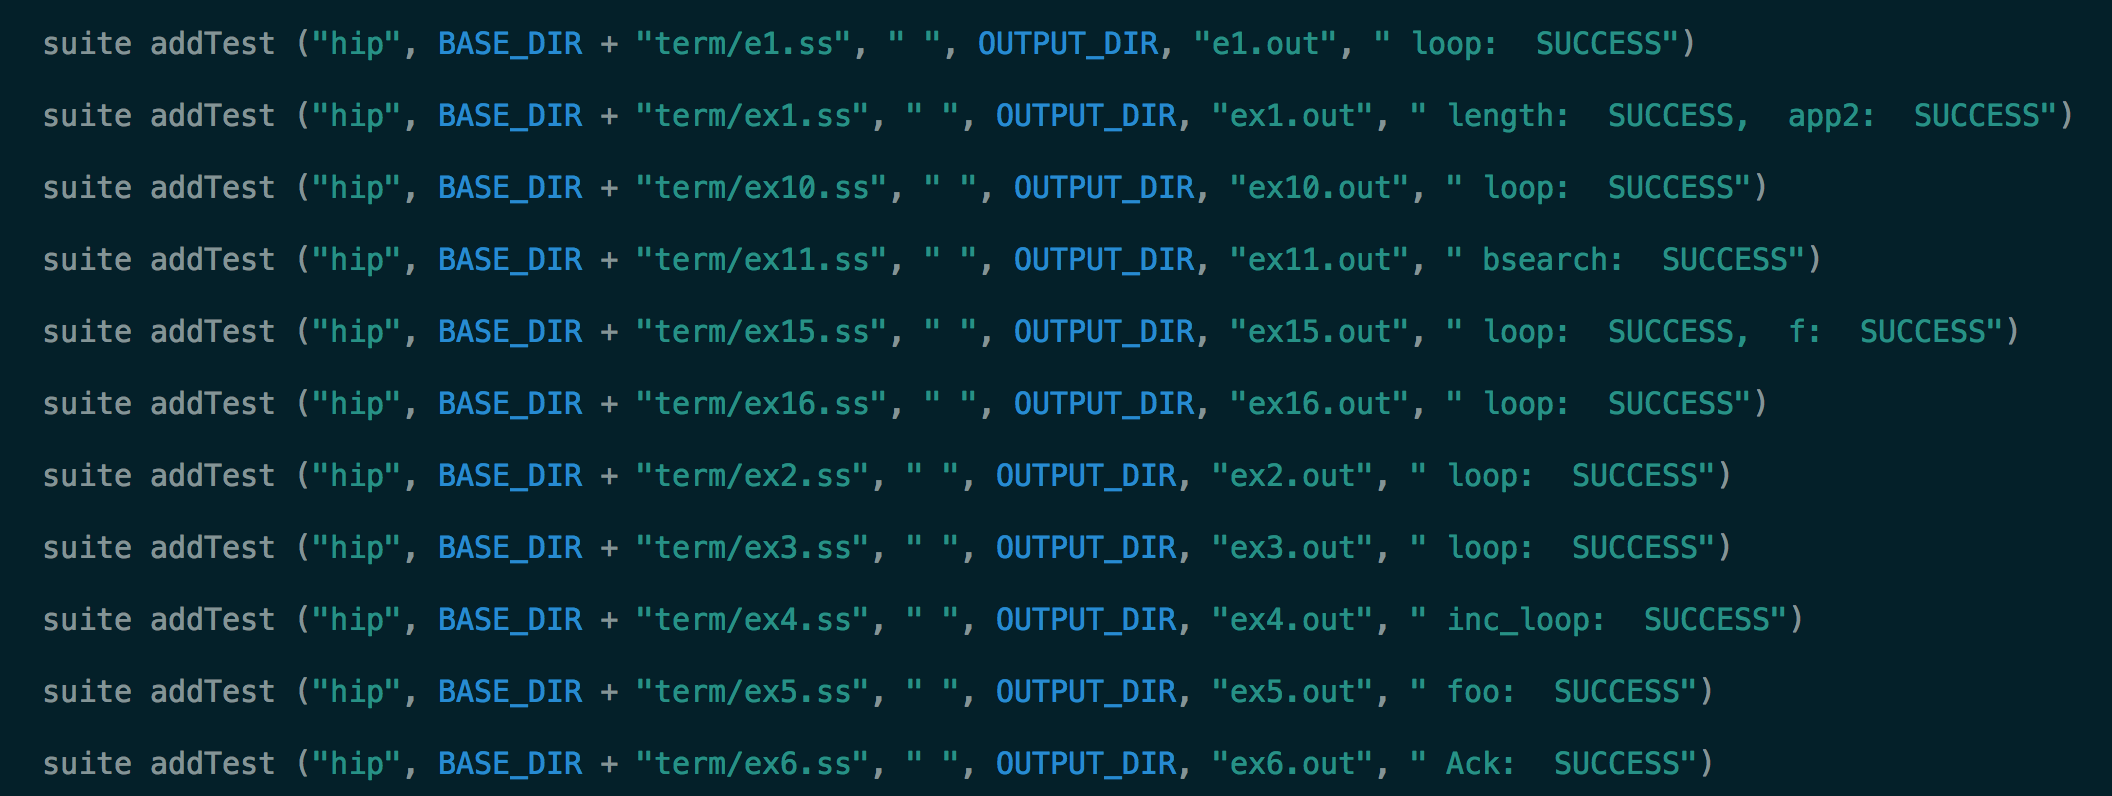
\includegraphics[width=320px]{figures/DSL_test_suite.png}
  \caption{Test Suite Creation}
\end{figure}
\end{frame}

\begin{frame}{Advantages of New System}
\begin{itemize}
\item Extensibility
\item Ensured Type Safety \cite{scala}
\item Highly Configurable
\item Lightweight Library
\item Easy to use
\item Domain Semantics \cite{dslsInAction}
\item Integration with Version Controlled Work - flow
\end{itemize}
\end{frame}

\begin{frame}{Project Objectives}
\begin{itemize}
\item Evaluate different DSL development techniques
\item Choose most applicable technique
\item Fulfill functional requirements of System Testing DSL
\end{itemize}
\end{frame}


\begin{frame}{Research Methodology}
\begin{figure}[H]
  \centering
    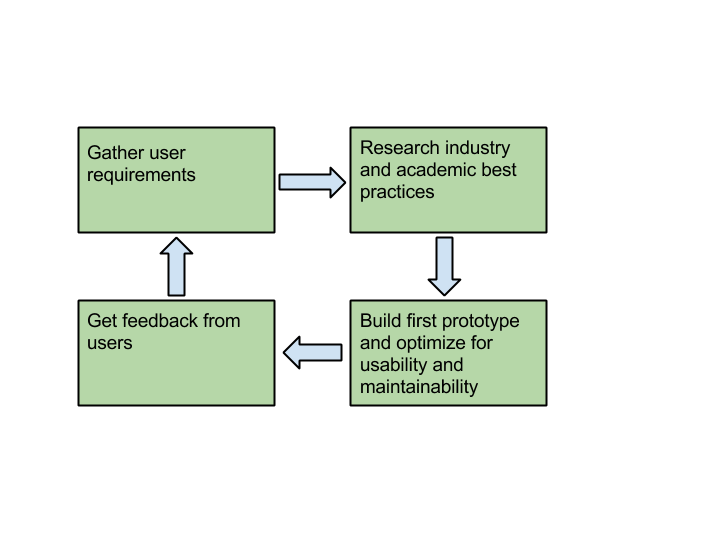
\includegraphics[width=300px]{figures/research.png}
  \caption{Research Methodology}
\end{figure}
\end{frame}
